
% Cal Poly Thesis
% 
% based on UC Thesis format
%
% modified by Mark Barry 2/07.
%

\documentclass[12pt]{ucthesis}

\usepackage{ifpdf} 
\newif\ifpdf
\ifx\pdfoutput\undefined
    \pdffalse % we are not running PDFLaTeX
\else
\pdfoutput=1 % we are running PDFLaTeX
\pdftrue \fi

\usepackage{url}
\usepackage{multicol}
\ifpdf

    \usepackage[pdftex]{graphicx}
    % Update title and author below...
    \usepackage[pdftex,plainpages=false,breaklinks=true,colorlinks=true,urlcolor=blue,citecolor=blue,%
                                       linkcolor=blue,bookmarks=true,bookmarksopen=true,%
                                       bookmarksopenlevel=3,pdfstartview=FitV,
                                       pdfauthor={Brett Armstrong},
                                       pdftitle={Can Clustering Improve Requirements Traceability?},
                                       pdfkeywords={thesis, masters, cal poly}
                                       ]{hyperref}
    %Options with pdfstartview are FitV, FitB and FitH
    \pdfcompresslevel=1

\else
    \usepackage{graphicx}
\fi

\usepackage{hyperref}
\hypersetup{
	linktoc=all,
    colorlinks,
    citecolor=black,
    filecolor=black,
    linkcolor=black,
    urlcolor=black
}



\usepackage{titlesec}
% \titleformat{\chapter}[display]% OLD
%     {\normalfont\huge\bfseries}{\chaptertitlename\ \thechapter}{20pt}{\Huge}% OLD
% \titlespacing*{\chapter}{0pt}{50pt}{40pt}% OLD
\titleformat{\chapter}[display]% NEW
    {\normalfont\centering}{\chaptertitlename\ \thechapter}{12pt}{}% NEW
\titlespacing*{\chapter}{0pt}{30pt}{20pt}% NEW

%\titleformat{\section}[block]{first}{label}{12pt}

\titleformat{\section}{}{\thesection}{1em}{}
\titleformat{\subsection}{}{\thesubsection}{1em}{}
\titleformat{\subsubsection}{}{\thesubsubsection}{1em}{}
\titleformat{\paragraph}{}{\theparagraph}{1em}{}

\usepackage[font={}]{caption}

%\renewcommand{\cftchapleader}{\cftdotfill{\cftdotsep}} % for chapters
%\renewcommand{\cftsecleader}{\cftdotfill{\cftdotsep}} 


\usepackage{amssymb}
\usepackage{amsmath}
\usepackage[letterpaper]{geometry}
\usepackage[overload]{textcase}
%\usepackage[toc,page]{appendix}

\usepackage{tabularx}
\usepackage{algorithm}
\usepackage{algpseudocode}

\usepackage{enumitem}
\setlist{nolistsep}


\floatstyle{boxed}
\restylefloat{table}

\bibliographystyle{abbrv}

\setlength{\parindent}{0.25in} \setlength{\parskip}{6pt}

\geometry{verbose,nohead,tmargin=1.25in,bmargin=1in,lmargin=1.5in,rmargin=1.3in}

\setcounter{tocdepth}{2}


% Different font in captions (single-spaced, bold) ------------
%\newcommand{\captionfonts}{\small\bf\ssp}
\newcommand{\captionfonts}{}

\makeatletter  % Allow the use of @ in command names
\long\def\@makecaption#1#2{%
  \vskip\abovecaptionskip
  \sbox\@tempboxa{{\captionfonts #1: #2}}%
  \ifdim \wd\@tempboxa >\hsize
    {\captionfonts #1: #2\par}
  \else
    \hbox to\hsize{\hfil\box\@tempboxa\hfil}%
  \fi
  \vskip\belowcaptionskip}
\makeatother   % Cancel the effect of \makeatletter
% ---------------------------------------



\begin{document}

% Declarations for Front Matter

% Update fields below!
\title{Toward General Purpose 3D User Interfaces: Extending Windowing Systems to 
Three Dimensions}
\author{Forrest Reiling}
\degreemonth{June} \degreeyear{2014} \degree{Master of Science}
\defensemonth{June} \defenseyear{2014}
\numberofmembers{3} \chair{Professor Zo{\"e} Wood, Ph.D.,\newline Department of Computer Science} \othermemberA{Professor Chris Lupo, Ph.D.,\newline Department of Computer Science} \othermemberB{Professor Franz Kurfess, Ph.D.,\newline Department of Computer Science} \field{Computer Science} \campus{San Luis Obispo}
\copyrightyears{seven}



\maketitle

\begin{frontmatter}

% Custom made for Cal Poly (by Mark Barry, modified by Andrew Tsui).
\copyrightpage

% Custom made for Cal Poly (by Andrew Tsui).
\committeemembershippage

\begin{abstract}
Recent growth in the commercial availability of consumer grade 3D user interface devices like the Microsoft Kinect and the Oculus Rift, coupled with the broad availability of high performance 3D graphics hardware, has put high quality 3D user interfaces firmly within the reach of consumer markets for the first time ever. However, these devices require custom integration with every application which wishes to use them, seriously limiting application support, and there is no established mechanism for multiple applications to use the same 3D interface hardware simultaneously. This thesis proposes that these problems can be solved in the same way that the same problems were solved for 2D interfaces: by abstracting the input hardware behind input primitives provided by the windowing system and compositing the output of applications  within the windowing system before displaying it. To demonstrate this it presents a novel Wayland compositor which allows clients to create 3D interface contexts within a 3D interface space in the same way that traditional windowing systems allow applications to create 2D interface contexts (windows) within a 2D interface space (the desktop), as well as allowing unmodified 2D Wayland clients to window into the same 3D interface space and receive standard 2D input events. This implementation demonstrates the ability of consumer 3D interface hardware to support a 3D windowing system, the ability of this 3D windowing system to support applications with compelling 3D interfaces, the ability of this style of windowing system to be built on top of existing hardware accelerated graphics and windowing infrastructure, and its ability to support unmodified 2D interface applications windowing into the same 3D windowing space as the 3D interface applications. This means that application developers could create compelling 3D interfaces with no knowledge of the hardware that supports them, that new hardware could be introduced without needing to integrate it with individual applications, and that users could mix whatever 2D and 3D applications they wish in an immersive 3D interface space regardless of the details of the underlying hardware.


\end{abstract}


\begin{acknowledgements}

Thanks to:

\begin{itemize}
\item My advisor Zo{\"e} Wood, for all of her guidance and wit.
\item The wonderful people in the Wayland and QtWayland communities, without whom I would not have a functioning prototype.
\item My parents, my family, and my girlfriend Katy, for supporting me always.
\end{itemize}

\end{acknowledgements}

\tableofcontents

\listoftables

\listoffigures

\end{frontmatter}

\pagestyle{plain}

\renewcommand{\baselinestretch}{1.66}


% ------------- Main chapters here --------------------
\chapter{Introduction}
The space we exist in is three dimensional, and this pervades every aspect of our interaction with reality. Everything we touch, see, and hear behaves according to the rules of this three dimensional space and this has made humans exceptionally proficient at reasoning about it, navigating through it, and modelling the behaviour of things within it. Yet when we interact with our computers, an increasingly important part of our everyday lives, most of us do so exclusively through two dimensional user interfaces. 
 
\section{Two Dimensional User Interfaces}

The two dimensional space in which we interact with computers has come to define these interactions in the same way that the three dimensional space in which we exist defines our interaction with reality. We use our fingers or a mouse press 2D buttons and open 2D menus, driving change in the application’s 2D interfaces which the windowing system composites into a 2D image to be sent to a 2D display. While this is natural for some intrinsically 2D concepts, like documents and images, other concepts which have no intrinsic spatial embedding, like file systems and networks, are also embedded in 2D when they are presented to the user in order to allow users to reason about them spatially. Even in applications which are intrinsically 3D, like physical simulation and modelling tools, the 3D application space is disjoint from the space in which the user exists (by necessity, since the application has no knowledge of the 3D relationship between the display and the user) and interaction between the 3D application space and the 3D user is traditionally done with 2D input events and 2D images.  
	
The flat nature of contemporary graphical user interfaces has come to define not just the way we interact with applications, but has also become an important factor in the physical design of the computers that run these applications. This is particularly apparent in the mobile computer space, where cost, weight, display power, and mobility concerns push devices toward ever smaller physical profiles, while usability concerns drive the devices toward larger interface surfaces, leading the profile of mobile computers to become flattened against their displays, with the devices acting as a physical embedding of the 2D computer interface within the 3D space in which the computer exists. This forces users to make a tradeoff between the physical profile of their device and the usable size of their interface; larger displays drive up mass both directly and through the need for a larger battery to meet increased power demands, but a smaller displays limit the usable size of the human-computer interface which limits the usability of the device [citation needed]. In desktop computers the same tradeoff must be made, because even absent power and weight concerns the size of the interface is still constrained by the cost of the displays and the physical space needed to mount them in view of the user.

Two dimensional user interfaces are certainly not all bad. There is a natural analog between interacting with documents, images, and folders on a desk and interacting with their digital counterparts on a 2D display (which forms the underpinnings of the familiar desktop metaphor). 2D interfaces also map well onto commercially available display hardware as a result of the two co-evolving for several decades, which keeps the hardware cost of 2D interfaces relatively low. 2D interfaces are mature and well studied, and there is a rich software ecosystem surrounding them which includes sophisticated, full featured user interface toolkits and advanced windowing systems, as well as a broad set of end user applications that provide 2D graphical frontends for almost every task a user need perform on a computer. Users are also familiar with the operation of 2D interfaces, which greatly reduces the time needed for users to learn new applications and improves their productivity with existing applications. 

There are certain applications, like document and photo editing and command line interaction, which fit well with 2D interfaces, and in these applications moving away from 2D interactions would likely be detrimental. However, many applications are intrinsically 3D, or are not intrinsically spatial at all and are embedded in a 2D space because it is simple and well supported, and a transition to 3D interaction has the potential to greatly improve  the usability of such applications \cite{bowman_theory_practice}.

\section{Three Dimensional User Interfaces}

The hardware, software, and theory surrounding high quality 3D human-computer interaction has been the subject of academic research for many decades, and the improved spatial reasoning this provides has been demonstrated to improve usability in a  number of applications  \cite{bowman_theory_practice}. 3D user interfaces are a broad group of interaction paradigms, including everything from desktop 3D modeling with a mouse and keyboard to fully immersive virtual reality.  This thesis focuses on ‘immersive’ 3D interfaces, which is used here to refer to 3D interfaces in which the user perceives the 3D interface elements to be in the same 3D space as their body, and has some way of manipulating these interface elements in 3D with corresponding 3D motion by some part of their body.  The hardware needed to support these types of interfaces has traditionally been very expensive, but recent technological improvements in a number of fields have brought many of the core hardware technologies onto the consumer market, bringing both high quality 3D input devices and immersive 3D displays into the reach of everyday computer users.

\subsection{Three Dimensional Input Devices}

Early 3D input devices to come into the consumer 3D interaction market were largely marketed as video game accessories, though their availability has led to their use in a wide variety of other application. These devices can be broadly categorized into two groups: devices which resolve the position and/or orientation of an element held or worn by the user, and range-imaging cameras, which produce a 3D image of a passive scene which contains no sensing elements itself.

The first category had its first commercial success in consumer markets in 2006, when Nintendo introduced the Wii Remote, or ‘Wiimote’, as the primary controller for its new Wii entertainment system. This controller, unlike traditional game console controllers, was able to sense its position, orientation, and acceleration along 3 axes. The Wiimote provided limited 3D control within Wii games, and was soon adopted by developers for a wider variety of tasks, including controlling the visualization of volumetric medical data \cite{wiimote-medical} and enabling head tracking 3D on traditional displays \cite{hacking-the-wiimote}. Several devices which provided similar input using a variety of different tracking technologies soon came to market, including Sony’s “Playstation Move” in 2009, and the “Razer Hydra” in 2011 (Produced by Sixense Entertainment in partnership with Razer USA). Until the time of this writing all commercially available, consumer grade, 3D tracking solutions have been handheld controllers gripped by the user, but two new multi-sensor, wearable, full-body tracking solutions (Sixense’s new magnetic tracking system, STEM, and PrioVR’s inertial tracking system) are due to become commercially available within the next year in response to an emerging consumer virtual reality market.
 
Range imaging cameras can be based on a variety of technologies, many of which have been commercially available for many years but have been too expensive to be accessible to a wide body of consumers. In 2009, following advances in real-time structured-light 3D scanning by Primesense Ltd, Microsoft released a range imaging camera based on a Primesense sensor to the public, under the name ‘Kinect’, as an accessory for their Xbox 360 game console. Designed to perform full body tracking in 3D on multiple users, the Kinect enabled a variety of new interaction techniques in Xbox games. Like the Wiimote, the Kinect was quickly adopted by third party developers and applied to numerous non-gaming domains, including robotics applications like Simultaneous Location and Mapping \cite{iser-rgbd-slam}, and a variety of medical applications \cite{kinect-medical}. Although the Kinect has received a great deal of attention, being the first consumer grade sensor capable of producing high quality images in real time, many other sensors have since come to market which offer comparable or better performance in a variety of applications and operating conditions. Primesense Ltd., the company that developed the technology underpinning the first generation Kinect, also developed sensors based on the same technology that were released both directly by Primesense under the name Carmine, and through Asus as the Xtion  and Xtion Live, which all offer very similar performance to the first generation Kinect \cite{depth-sensor-comparison}. Very recently, several consumer-grade range imaging cameras have become commercially available which rely on ‘time-of-flight’ technology, which has several advantages over structured lighting including lower software overhead, faster response time, and better bright light performance \cite{ti-tof}. This includes Microsoft’s next generation Kinect, released with the Xbox One in 2013, and the DS310 and DS325 from Belgium based SoftKinetic. The SoftKinetic DS325, also sold re-branded as the Creative Senz3D, is designed for close interaction and finger tracking rather than full body tracking \cite{softkinetc-products}, and competes in the consumer market with the Leap Motion, a desktop stereo camera designed specifically for hand, finger and stylus tracking in the space immediately above the keyboard. Several other companies, notably Texas Instruments and pmdVision, provide Time of Flight solutions, but to the author’s knowledge they do not sell consumer time of flight products as of the time of this writing. 
This is by no means an exhaustive list of 3D input devices; it is meant only to demonstrate the growing diversity of 3D input devices reaching the consumer market, and that this is a relatively recent development. At the surface level, these devices appear to produce a wide variety of input, but when constrained to human-computer interaction applications it becomes apparent that simple input models can capture the useful input produced by all of these devices. Essentially this is because the only mechanism humans have to produce 3D input is the movement of their body through the 3D space or the use of this movement to move an object through 3D space, which can be captured, respectively, by the notions of skeletal tracking and 3D pointing devices [cite Jester].

\subsection{Immersive Three Dimensional Displays}
	
	The term "3D display" has come to refer to a very broad category of devices, so the term "immersive 3D display" is used here to refer to graphical displays which support both stereo parallax (rendering the scene from a separate viewpoint for each eye) and head-tracking motion parallax (adjusting the position and orientation of these viewpoints based on the 3D relationship between the user and the display), as both are required to create a convincing 3D experience for the user (This is discussed in more detail in the background section). This excludes commercial 3D televisions and 3D movie theaters because they do not provide head tracking, and excludes haptic and audio ‘displays’ because they are not graphical. There have been many systems which meet these requirements in research and industrial applications, including Responsive Workbenches [citation], Hemispherical Displays [citation], CAVE Automated Virtual Environments (CAVEs) [citation], and Head Mounted Displays (HMDs) [citation], and some of these technologies, particularly CAVEs and HMD’s, have received significant research and developments, allowing the technology to mature significantly. 
Most of these technologies have remained outside of consumer reach, largely due to the large size and high cost of such systems, with the exception of HMDs, whose simplicity and compact design has led them to enjoy intermittent commercial availability for many years. A comprehensive discussion of commercially available HMDs is outside the scope of this paper, but it is worth noting that the recent release of OculusVR’s ‘Oculus Rift’ development kit to consumer markets has sparked a resurgence in interest in virtual reality for video games and other entertainment applications, leading to the announcement of several new consumer HMDs, including a consumer version of the Oculus Rift [citation], Sony’s ‘Project Morpheus’ [citation], and True Player Gear’s ‘Totem’ [citation]. 

Priced at only a few hundred dollars, these HMDs put high resolution, wide field-of-view, immersive 3D display technology in the hands of everyday computer users, and the continuing advances of consumer graphics processing hardware gives them the ability to drive convincing 3D scenes onto these displays with commodity hardware. Furthermore, like 3D input devices, the similarity in function between these devices means their behavior can be captured abstractly by relatively simple input and output models. 

\chapter{Motivation}
The recent influx of commercially available 3D input devices and immersive 3D displays to the consumer market, coupled with high performance consumer graphics hardware, has given end users access to all of the hardware needed to support high quality, immersive 3D human-computer interaction for the first time ever. However, current application support of this kind of hardware is very limited, consisting mainly of demo applications and video games, and applications which support more than one of these devices are even more rare. 

\section{Obstacles Facing the Adoption of 3D Interfaces}

In general, immersive 3D user interfaces require both a good 3D input device and an immersive 3D display, and with such limited device support it is rare that an application supports both and even more rare that an end user will own a 3D input device and an immersive 3D display which are both supported by the 3D user interface application they wish to use (much less every 3D user interface application they wish to use). This problem could be attributed to many factors, including that it is too early in the life of these devices for applications to have been developed, or that there is simply limited application potential for this these devices. And while these certainly could be contributing factors, there are also tangible shortcomings in the software ecosystem surrounding this new hardware which indicate that this problem is not simply going to go away on its own.

\subsection{Device Abstraction}

The first problem to become immediately apparent is the sheer diversity of 3D interface devices, a problem which will only get worse as more and more devices come to market. There is a fair amount of similarity within these devices, and the even greater similarity within the actual 3D interface primitives which each is actually capable of providing. Every 3D input device discussed above provides either some information about the 3D pose of the users body [cite Jester] or the 3D transform of some kind of handheld device, and immersive 3D displays all serve the same purpose of giving the user a sense of presence in a virtual (or mixed reality) 3D space. Despite this, there is no widely adopted abstraction for either 3D input devices or immersive 3D displays, and while some such abstractions exist, each has its own unique shortcomings (this is discussed further in the related works section). 

Rather, every one of these devices comes with its own API, designed to work with that device and usually other devices from the same manufacturer. If an application wishes to use this device it must be ported to use that device’s API, and if it wishes to be compatible with multiple devices in the same class from different manufacturers it must include dedicated code for each of the devices it wishes to support, and this code must be maintained by the developers of each application independently. Support for devices can be abstracted by a user interface toolkit like Vrui \cite{vrui}, a video game engine like Unity or Unreal (via vendor provide plugins), or even a dedicated abstraction libraries like MiddleVR \cite{middle-vr} or VRPN \cite{vrpn}. Each of these has its own strength and weaknesses, but there are also overarching shortcomings of including the abstraction layer in toolkits used on a per application basis. First, this means that the device abstraction layer has to be replicated for each toolkit (causing the same problems as replicating it for each application). This could hypothetically be resolved by the uniform adoption of a single toolkit which meets the need of every application needing a 3D user interface, but given the wide variance in demands between something like a 3D file browser and an immersive VR experience, this seems both unrealistic and, in the author’s opinion, very much undesirable. Secondly, if the abstraction is done within toolkits used on a per application basis, then two applications using different toolkits (or perhaps even the same toolkit) that attempt to use the same device simultaneously could block one another from accessing the device. This is closely related to the next major problem with the software ecosystem surround 3D user interface devices.

\subsection{Multiple Application Support}

The ability to use multiple applications simultaneously has become a core feature of the interface paradigms we use today, and the ability of a user to install and run together whichever set of applications they like is the key point of software modularity that has allowed personal computers to be useful to a broad class of users with highly diverse requirements.
 
This same point of modularity can be applied to 3D user interfaces, and to a certain extent it already is. It is certainly possible to install multiple 3D user interface applications and, depending on the applications, maybe even run them simultaneously. However, there are serious limitations here as well, particularly when it comes to immersive 3D displays. These displays require custom projection of a 3D scene for each eye, and this projection must be consistent with the 3D position of the users head relative to this scene and the display surface, and many HMDs require a post-projection adjustment to correct for distortion introduced by the optical system (this is discussed in detail in the background section). While it is relatively straightforward to implement this behavior in an application which draws itself (and only itself) to the entire display surface, sharing the 3D display between multiple applications with 3D user interfaces introduces significant problems.
The essential problem is that in order for the 3D interface space to be divided between multiple 3D interfaces from different applications in a meaningful way, it must be divided in 3D. This is difficult because current graphics and windowing infrastructure, as well as the 2D display technology underlying the immersive 3D display, is designed around the paradigm of applications producing 2D output which is combined in 2D by the windowing system and driven onto the 2D interface space of a traditional display. This works well for dividing the 2D space of a display among multiple 2D interfaces, since they can each be given a rectangular region of the rectangular display, but dividing the 2D display surface of an immersive 3D display among multiple 3D interfaces in the same way (without applying the correct stereo projection and optical distortion correction) produces results which do not appear to be in the same 3D space. 

This means that while an immersive 3D display can produce a compelling 3D interface space for a single application, it is not possible for multiple 3D interface applications to share the 3D display in the same way that 2D applications can share a 2D display. It also means that 2D applications which have no reason to need a 3D interface are also unable to use the immersive display, despite the fact that embedding a 2D interface surface in a 3D interface space is conceptually simple and well defined.

\section{Insights from Two Dimensional User Interfaces}

	The core goal of this thesis is derived from the simple observation that the problems currently facing the development of applications with 3D user interfaces and the integration of the hardware that supports them are present for 2D interfaces as well, with the key difference that in the domain of 2D interfaces these problems have already been solved. Despite the fact that the diversity of displays, mice, and keyboards dwarfs the diversity of 3D user interface devices, users are able to assemble a hardware interface from almost any combination of devices they like and run all of their favorite applications on top of their custom hardware interface. New 2D interface devices need not be integrated into every application that uses them, and multiple 2D interfaces from different applications can be used together in the same 2D interface space in arbitrary combinations. 
	
\subsection{Windowing Systems}

	Applications with 2D interfaces no longer suffer these problems is because modern consumer operating systems provide a set of 2D interface abstractions called a windowing system. Windowing applications do not interact directly with the mouse, keyboard, or display. Rather the windowing system manages input devices and displays (usually through lower level abstractions provided by the kernel), and provides the interface capabilities of these devices as services to applications. Applications receive input events like mouse movement from the windowing system abstractly without needing any knowledge of what type of mouse is used, how it is connected, or who manufactured it. The 2D images produced by applications are not drawn directly to the display, they are given to the windowing system which then composites the output of all running applications (sometimes in a separate compositor program, depending on the windowing system) into a final 2D image which is scanned out to the display itself. 
This basic system architecture is present, with slight variation, in every major graphical operating system. It is connected with the prevalent ‘Windows, Icons, Menus, Pointer’ (WIMP) interaction paradigm and the popular desktop metaphor, which are well understood, well tested, and familiar to users. This architecture has also strongly influenced the way applications interact with hardware accelerated 3D graphics systems, leading to a design pattern where applications are responsible for projecting their 3D content into a 2D image before delivering it to the windowing systems, and this has in turn influenced both the design of 3D graphics API’s as well as the hardware which underlies them. The ubiquity of windowing systems has also profoundly affected the high level topology of the software ecosystem surrounding WIMP interaction, leading to the emergence of user interface toolkits like QT and Java Swing that abstract popular windowing systems behind their common functionality so that sophisticated, cross platform, WIMP applications can be developed without knowledge of the underlying software mechanisms, much less the hardware devices, that support them.
 
Even existing 3D interface applications use the windowing system to abstract traditional input and to draw to the 2D display that underlies its immersive 3D display, but without the ability to abstract 3D input devices and to mix 3D interfaces in 3D, these windowing systems do not give applications the ability to share 3D interface hardware in a meaningful way.

\section{Proposed Solution: A Three Dimensional Windowing System}

The primary goal of this thesis is to demonstrate that windowing systems are capable of solving the some of the core problems facing 3D user interfaces in the same way that they have already solved the exact same problems for 2D user interfaces, and that this can be done with extensions to an existing windowing system, allowing both unmodified 2D applications and as device-agnostic 3D applications to window into the same 3D interface space. 

The type of windowing system described here extends the concept of a window as a 2D region of a 2D interface space to the 3D interface space provided by the 3D user interface hardware described above. It allows 3D applications to create a 3D analog of a traditional window, representing a 3D region of the 3D interface space which can be manipulated in 3D in much the same way as a traditional 2D window can be manipulated in 2D. These 3D windows can listen for 3D input events via the same mechanism that is used to listen to 2D input events, and the 3D output they produce is mixed in 3D with the 3D output of other 3D applications.

Additionally, this type of windowing system allows traditional, unmodified 2D applications to create a 2D interface context in this 3D windowing space which behave exactly the same as a normal window from the applications perspective. The windowing system embeds these 2D windows in the space in much the same way that a sheet of paper embeds a 2D document in 3D reality, allowing the user to manipulate and manage these windows as 3D objects. 3D input events managed by the windowing system are projected onto the 2D window before being delivered to the 2D application, allowing the user to send meaningful 2D input to the application with a 3D input device.

\subsection{Advantages of This Approach}

There are numerous advantages to solving these problems for 3D user interfaces in the same way that we solve them for 2D interfaces, a few of which are discussed here in detail. Some of these advantages are the same advantages that led to the adoption of windowing systems in the first place, and others are simply result from leveraging extensive work put into windowing systems for 2D interfaces. This is by no means meant to be an exhaustive list.

\subsubsection{Hardware Abstraction and Multiple Application Support}

This approach allows a hardware 3D interface (consisting of at least one immersive 3D display and at least one 3D input device) to support a unified 3D interface space, where both 2D and 3D applications are treated as first class components of the human-computer interface and managed together in the 3D space via a unified window management mechanism. 

This means that any hardware capable of supporting the 3D windowing system can support all 3D applications which use it (as is the case with 2D applications), and that new hardware need only provide a driver for the windowing system abstraction to achieve support from all applications using the system (as is also the case with 2D interfaces). 

It also means that the structure of the software ecosystem surrounding 2D WIMP interaction can be applied to the software ecosystem surrounding 3D interfaces, allowing the development of a wide variety of user interface toolkits which provide high-level, domain-specific interaction metaphors built on top of common abstractions provided by the windowing system, allowing multiple applications using different toolkits (or no toolkit at all) to share the 3D interface hardware supporting the system in a meaningful way. Furthermore, because the system supports unmodified 2D applications, support for 3D interface elements could even be integrated into existing 2D interface toolkits where appropriate.

\subsubsection{Compatibility With Existing Graphics and Windowing Infrastructure}

	As the provided implementation demonstrates, it is possible to support compositing 3D content in a 3D space while only needing to send 2D images from the application to the windowing system. This means that existing, full-featured 3D graphics API’s, which give the application full control over every aspect of how its 3D content is drawn into a 2D image, are still perfectly well suited to this task. This means that applications retain full flexibility in what they draw and how they draw it, and can still benefit from acceleration by high performance consumer graphics processing units (GPUs). It also means that 3D applications still benefit from the extensive software infrastructure that has been put in place to allow 2D applications to efficiently pass 2D images to the windowing system and to allow the windowing system to composite these images off screen. Together this means that the 3D windowing system can efficiently support both 2D and 3D applications without needing to lay extensive new infrastructure to do so.

\chapter{Contribution}
The primary contribution of this work is an open source implementation of a 3D windowing system built on top of the Wayland display server protocol. It is intended both to demonstrate that windowing systems can solve some of problems hindering the adoption of 3D user interfaces, as well as to provide a body of code capable of forming the core of a functioning, full featured, open source 3D windowing system. 
	
This implementation includes the Wayland protocol extensions necessary to enable 3D windowing, a framework for building Wayland compositors which support these extensions (built on top of the QtWayland Compositor library), an example compositor which uses this framework to support the windowing system on top of the Oculus Rift Developer Kit HMD and the Razer Hydra motion controller, drivers for these devices, a client side library for handling the protocol extensions and graphics trickery needed for 3D windowing, and a few example clients which  demonstrate how to use the client side library. 

This software demonstrates the ability of consumer 3D interface hardware to support a 3D windowing system, and the ability of this 3D windowing system to support applications with compelling 3D interfaces. It also demonstrates that this style of windowing system can be built on top of existing graphics and windowing infrastructure, and that if can support unmodified 2D applications windowing into the same 3D interface as the 3D applications. 

This implementation is not intended to be release quality by the completion of this thesis, and it is not intended to embody all of the functionality which such a windowing system could hypothetically provide, particularly when it comes to device abstraction. Rather, it is intended to show what is possible, and provide the core functionality needed in a piece of software which is modular enough to form the core of a comprehensive, open source solution. 

\chapter{Related Works}

Both windowing systems and 3D user interfaces have received a great deal of research over the past few decades, and these fields intersect in a number of ways, so placing this thesis within existing research is somewhat complicated. 

The system described in this paper has the key design goal of being able to seamlessly handle both 2D and 3D interface contexts in the same 3D interface space, so we will compare it to existing research based on this. This primary design goal can be broken down into several secondary goals, including allowing applications to request 2D and 3D windows in the same manner, allowing users to interact with 2D and 3D windows in the same manner, and allowing applications to receive 2D and 3D input in the same manner. Other design goals include allowing applications to use the windowing system without needing to be started by it and allowing 2D applications to window into the 3D space without needing to be modified. To the author's knowledge this set of requirements is not met by any system in existing research.

\section{Two Dimensional Windows in Three Dimensional Environments}
A fair amount of work has been done on managing traditional 2D windows in a 3D space, both in research and, more recently, in production software. These systems can handle multiple 2D windows in a 3D space and can draw the 2D output of a 3D application as a 2D window, but none of them provide a mechanism for unifying the application space with the windowing space for seamless 3D interaction between multiple applications in a single 3D space.

The Task Gallery \cite{task_gallery} is a 3D window manager for Microsoft Windows which embeds groups of related windows called 'tasks' into a 3D space to make them appear like artwork hung in a gallery, with the active task on a center 'stage'. This system has some truly 3D user interface elements, like the gallery and the stage, but it exclusively supports 2D windows. 

Topol describes a system for embedding standard X11 windows into a 3D workspace using techniques similar to those used by modern compositing window managers \cite{xwindow_immersion}. However, like The Task Gallery, this system supports only flat, 2D windows. Additionally, it does not appear that this system support mapping input from the 3D workbench space into the 2D window space.

Feiner et al. demonstrate a similar 3D window management system in an augmented reality setting with their Windows on the World system \cite{wotw}. This system uses a very large X bitmap which applications draw into using traditional means. The display server displays a small portion of this bitmap at a time on a see through head mounted display, and determines which portion of the bitmap to draw into by mapping the pitch and yaw of the user's head onto the x and y coordinates of the bitmap, thereby mapping the bitmap onto a portion of a spherical surface surrounding the users head. Windows can be moved within the bitmap such that they always track the projection of a real world object onto the spherical surface, thereby creating the illusion that the window is attached to that object.
 
\subsection{In Production Software}

As GPU accelerated window compositing has become widely available on consumer hardware (following improved OpenGl support in X.org around 2006) the ability to handle windows in 3D has become broadly available in consumer software.  Some widely used compositing window managers, like Compiz \cite{compiz}, draw window output as textures on 2D surfaces in 3D, allowing them to create compelling 3D visual effects and animate window transitions in 3D space. However, because the architecture of X11 does not give the compositor control of the input system, X11 compositing window managers like Compiz are unable to properly redirect input to the windows while their output is transformed to appear 3D, which seriously limits ability X compositors to create useful 3D interfaces.

The open source community has been seeking to address many of the problems and shortcomings of X11 with the development of a completely new display server protocol called Wayland \cite{wayland}. One of the key differences between Wayland and X is that the display server and the compositor are the same entity, meaning that the compositor can both transform window output to appear embedded in a 3D space while also mapping 3D input back into the 2D window space, allowing traditional 2D windows to be first class citizens of new 3D user interfaces. This, coupled with the simplified architecture of Wayland, is the reason why Wayland forms the basis of the windowing system presented in this thesis.

There are other production windowing systems which allow output from windows to be transformed to appear 3D, used mainly to provide 3D window transition effects like Flip 3D in Windows Vista and Windows 7. To the author's knowledge no production window manager allows normal window interaction while the windows' output is transformed to appear 3D.

\section{Three Dimensional Windows}

There are systems in existing research which explore concepts similar to the 3D windows described in this paper. For the most part what separates them from the work in this thesis is lack of support for windowing by external applications, limitations on what clients are allowed to draw within their windowing volumes, or lack of first class support for 2D windows.

The earliest work (to the author's knowledge) which explores such a concept is Feiner and Besher's n-Vision testbed \cite{nvision} in 1990, a system designed to facilitate the visualization of high dimensional data using a hierarchy of nested 3D visualization volumes called 'boxes'. Each box draws a 3D slice of the multidimensional space by mapping the high dimensional function across 2 selected independent variables within the box, with all other independent variables held fixed within the box at a value determined by the box's position within its parent box. This nested hierarchy of boxes is much like a 3D analogue of the X protocol's hierarchy of 2D rectilinear windows (as the authors note), but it is not designed to allow third party applications to create such volumes and draw content inside of them. It also lacks support for 2D windows, and the capabilities of the system appear to be limited to graphing multivariate functions.

DiVerdi demonstrates a 3D augmented reality window manager called ARWin \cite{arwin} which he uses to manage 3D user interface elements and 2D windows in his Anywhere Augmentation system \cite{anywhere-augmentation}. It is difficult to firmly compare this thesis to ARWin because the description of ARWin does not go into great detail about the system's implementation. One difference that is clear is that the system lacks native support for 2D windows, instead supporting 2D windows through a VNC client which outputs the windows content to a texture (which limits 2D support to applications without hard latency requirements). While their system supports multiple applications drawing 3D user interface elements in the same 3D space, it is not clear what constraints are imposed on this process or the mechanism by which 3D applications draw content in the 3D space. It is also unclear how applications request a session with the display manager, and even if this is possible without the display manager starting the application itself. No documentation regarding the windowing mechanism could be found.

\section{The Three Dimensional Workspace Manager (3DWM)}

The system in existing research which appears to be the closest thing to the system described in this thesis is 3DWM \cite{3dwm}, a system designed to provide a network transparent hardware abstraction layer for 3D user interfaces and a reusable 3DUI toolkit to ease the development and research of new 3D user interfaces. Like the system described in this thesis (and like the X Window Protocol and the Wayland display server protocol) the basic system architecture consists of a display server which manages the input and output hardware, and a set of independent client applications which are able to request that the display server notify them of input events and draw content for them on the output hardware. 

Unlike the system described here, but much like early uses of X, their display server draws user interface primitives on the behalf of the client and does not allow the clients to directly control the way the primitives are drawn. This is done because (like early X) network transparency was one of their core design goals, and transmission of pixel buffers from real-time graphics applications to the display server requires much greater bandwidth and much lower latency than most networks are able to provide. The system described in this thesis avoids this (by sacrificing network transparency) because although it gives the system a unified look and feel, it requires that applications perform many transactions with the display server in order to accomplish basic user interface tasks and limits the behaviour and appearance of application user interfaces to functionality supported by the display server. These are the same factors which led to the abandonment of the widespread use of X11's primitive drawing capability and the loss of its pure network transparency (through the use of direct rendering extensions to X) and are two of the major factors motivating the development of Wayland as a replacement for X. 

3DWM does support multiple application contexts in a single 3D space, and allows applications to request volumes for their personal use, which is very similar to the concept of 3D windows presented in this thesis (and is compared to the concept of windows by the authors). However, unlike traditional windows, and unlike the 3D windows presented in this thesis, client applications do not have full control of what is drawn inside of their windowing context. Instead, clients are only able to request that the display server draw primitives inside of their volume, and if the primitives the display server provides do not meet the needs of the application then the developers have no choice but to modify the display server.

Another shortcoming of 3DWM is the lack of native support for 2D windows inside the 3D application space. While the need to support 2D applications is not ignored completely, it is viewed as 'legacy' support during a 'transitionary phase' to completely 3D interfaces and as such 2D applications are not treated as first class clients of the display server. Instead, they implement a custom VNC client which writes a remote desktop into a texture which the display server then applies to a surface in the 3D space. While this does indeed provide simultaneous support for 2D applications running on many platforms, it does not allow individual 2D and 3D applications to be mixed and used together in the same 3D space. 

\chapter{Technical Background}
Understanding the design and implementation of the windowing system presented in this thesis requires understanding of some technical, domain-specific concepts which may be outside the knowledge base of some readers, so this section is included to consolidate and summarize these concepts. An in-depth discussion of most of these concepts is well outside the scope of this thesis, but references to more detailed explanations are provided where possible. No novel material is presented here, and readers familiar with computer graphics and open-source windowing systems could certainly skip this section altogether.

\section{Computer Graphics}
The demands of computer graphics applications are fundamentally very different from many other applications, and this has led to the development of specialized hardware coprocessors for accelerating these types of applications called Graphics Processing Units (GPUs). Modern GPUs are programmable computers, much like the CPUs that control them, but they are massively parallel and every aspect of their design is oriented toward exceptionally high data throughput. GPUs are designed to execute a single program on many similar pieces of data in no particular order, making them well suited for computer graphics applications (where a substantial portion of the computational load lies in transforming vertices and shading pixels), as well as many other problems which map well onto the Single Program Multiple Data paradigm. Depending on the GPU manufacturer access to this hardware may be possible through several API’s, but for graphics applications on open source systems the API of choice is OpenGL.
		
OpenGL organizes access to graphics hardware around a data pipeline commonly referred to as ‘The Graphics Pipeline’, and while a detailed description of this pipeline is certainly beyond the scope of this thesis, some of its stages are very important to the design of the windowing system here, so a brief overview is included. Readers seeking further explanation are directed to [citation] for a good introductory overview of the modern graphics pipeline and [citation] for a very good and very in-depth discussion of its function. The modern graphics pipeline is complex, and many datapaths exist, but for the scope of this explanation we will focus on the primary datapath illustrated in Figure \ref{graphics-pipeline}.

\begin{figure}[ht!]
\centering
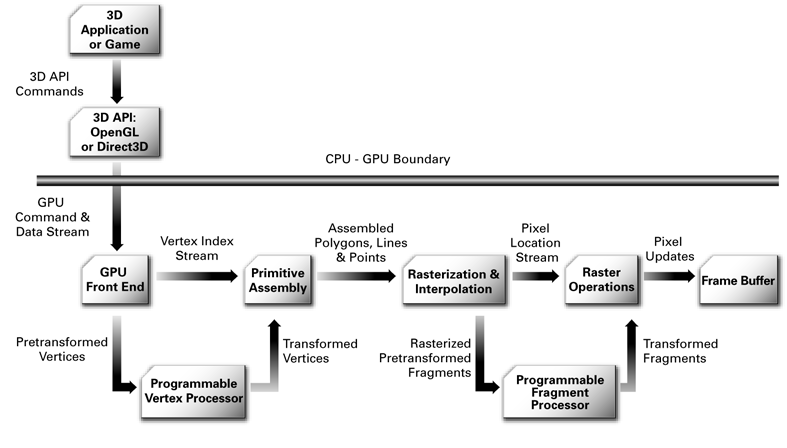
\includegraphics[width=1.0\textwidth]{images/graphics-pipeline.png}
\caption{The basic structure of the graphics pipeline. Note the vertex processor, rasterizer, fragment processor, and termination in a frame buffer. Image taken from  \protect\cite{litime}}
\label{graphics-pipeline}
\end{figure}


\subsection{The Vertex Transformation}
In this datapath, incoming geometry is first transformed in the vertex processor from the space in which it defined into the space in which it is projected onto the 2D output surface. This vertex transformation, shown in Figure \ref{vertex-transformation} is represented as the composition of several linear transformation matrices in a homogeneous coordinate space, which, being linear transformations, can be applied to the vertices in a sequence or as a composite transform computed as the outer product of the component matrices. Though in principle any number of transformations can compose this composite vertex transformation, it is typically thought of as being composed of three principal transformations. 

\begin{figure}[ht!]
\centering
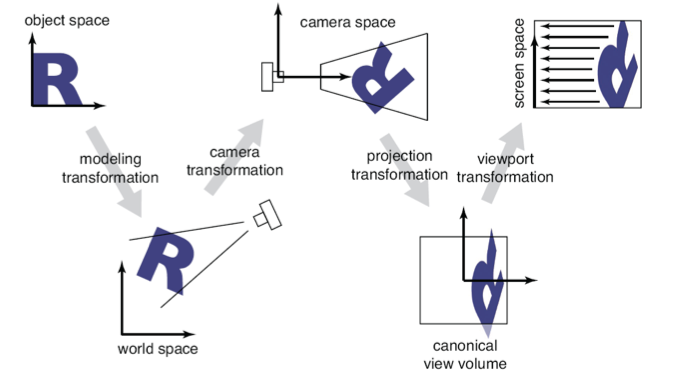
\includegraphics[width=1.0\textwidth]{images/vertex-transformation.png}
\caption{The basic sequence of transformations applied to geometry in the vertex processor. The final transformation in this sequence is applied after the vertex processor and is not part of the composite transformation matrix. Image taken from  \protect\cite{litime}}
\label{vertex-transformation}
\end{figure}


The geometry of an object is defined in a space relative to that object, which allows multiple copies of an object placed throughout a scene to share geometry on the GPU. The first transformation, called the ‘modeling transform’ or ‘model matrix’, maps geometry from object space into the space in which the scene is defined, called ‘world space’. The second transformation, called the ‘camera transformation’  or ‘view matrix’, maps geometry from world space into the space of the virtual camera, whose origin is the center of projection of the camera and whose axes are aligned with the camera’s view vectors. This is followed by the projection transformation, which (coupled with a hardware accelerated homogenous divide following output from the vertex processor) maps the vertices into ‘normalized device coordinates’, where all vertices lying inside the view frustum defined by the projection matrix now lie inside the ‘canonical view volume’ reaching from -1.0 to 1.0 along all axes of the new space.
Understanding how these transformations affect the user’s perception of 3D information is important because the synchronization of the matrices that represent them between the client application and the windowing system is the key to correctly compositing 3D clients without needing to do the projection within the windowing system. A simple example is included here to ensure this is clear to all readers.

\subsubsection{A Simple Example: Transformations}

Imagine we have a simple scene containing three objects, a table, a chair, and a room which contains them. Each of these objects has its own model transform, allowing us to move them around independently, but the view and projection matrices are global for all objects, reflecting the idea that there is only one camera. Translating the model matrix of the chair changes where the chair is projected onto the screen, but has no effect on the table or the room, which gives the appearance of the chair moving relative to the room and the table. Translating the view matrix, by contrast, changes how all three objects are projected onto the screen in the same manner. Because humans naturally contextualize the room as a static entity, given their experience with similar structures in reality, this translation gives the viewer the impression of their viewpoint moving through the space containing the objects. Changes to the projection matrix also affect the projection of all three objects, again giving us the impression of changing the properties of the virtual camera. For example, reducing the field of view encoded in the projection matrix affects the resulting image in the same way that a telephoto lense changes the image of reality produced by a real camera. 

\subsection{Rasterization and The Depth Test}
Following output from the vertex processor primitives (like points and lines) are assembled and clipped against the canonical view volume. A final transformation called the ‘viewport transform’ is applied, mapping the X and Y components of the normalized device coordinates into the screen space specified in pixels, and the primitives undergo a process called ‘rasterization’ or ‘scan conversion’, which determines which pixels are covered by the projection of the primitive. A data structure called a ‘fragment’ is generated for each pixel that lies inside the projection of the primitive, and all further stages of the graphics pipeline, including programmable fragment shaders, operate on these fragments. 

At this point we encounter the second concept which is critical to understanding the windowing system presented in this thesis. The vertices (and the primitives assembled from them) are three dimensional, but the screen space in which the fragments are specified is only two dimensional, and in the projection from three dimensions to two some information must be lost. More concretely, it is possible for one object to partially occlude another if it is closer to the camera, and in this case it is necessary that the we draw the closer object in front of the further one. To achieve this behavior the graphics pipeline includes a step called the ‘depth test’ which, depending on the behavior of the fragment shader, takes place either immediately before or immediately after a fragment is run through the fragment processor.

The depth test operates on a two dimensional scalar buffer called the ‘depth buffer’ attached to the active frame buffer which is of the same dimensions as the color buffer being drawn into. The depth of each fragment (the Z component of its position in the projection space) is compared to the depth currently stored in the depth buffer at the XY position of the fragment in question. If the depth of the current fragment is closer than the current contents of the depth buffer the current fragment is drawn, otherwise it is discarded. This guarantees that the closest fragment at a given screen position always determines the color at that position regardless of how many other fragments are drawn to the same screen position or in what order they are drawn. 
The depth buffer is critical to the function of the windowing system presented in this thesis because it can be used to composite the output of 3D applications in 3D using only 2D buffers in the same way that it is used to composite 3D primitives in the normal graphics pipeline (using the same hardware depth test no less), which allows a 3D windowing system to be built on top of windowing infrastructure designed to pass only 2D buffers from applications to the windowing system, and allows applications to use graphics API’s designed around the idea that applications control every aspect of how their 3D content is drawn down to the coloring of the pixels.
Frame Buffers

The termination of the graphics pipeline datapath is a frame buffer. The frame buffer itself is not actually a buffer, but rather a collection of handles for different kinds of buffers, like color buffers or depth buffers, to which actual buffers can be attached. While applications typically render to the ‘default framebuffer’, which represents their actual output to the windowing system (or, in the case of the windowing system, the output to the display), it is also possible for applications to create off-screen frame buffers called Frame Buffer Objects (FBOs) in order to perform multiple rendering passes. This concept is used extensively in the implementation of the windowing system presented here. 
	
\section{Open Source Windowing Systems}

Though the basic concept of windowing systems pervades all graphical operating systems, there are some architectural details of the windowing systems used in open source operating systems which are relevant to the windowing system presented in this thesis. This discussion will focus on X, which has been the predominant Linux windowing system for almost two decades, and its replacement, Wayland, which forms the foundation of the windowing system presented in this thesis.

\subsection{Basic Architecture}

These windowing systems are built around an architecture where a program called a ‘display server’ manages displays and input devices, and applications which desire a graphical interface context connect to the display server as clients via a standardized ‘display server protocol’. The names X and Wayland both technically refer to the display server protocol itself, and in both cases the protocol is extensible, allowing the windowing system to dynamically meet the needs of graphical systems as they change with technological development. This has largely allowed X to withstand the test of time, although the developers behind Wayland argue that the way X is currently used is so tangential to its original design goals that its function has largely degraded to providing “really bad IPC” [citation]. The effort to resolve these problems led to the development of Wayland, which, as the Wayland architecture page states, is most easily understood through comparison with X [citation].

\subsection{Wayland and X}

As with the other topics in this section, a thorough discussion of the architectural differences between Wayland and X is both outside the scope of this thesis and largely irrelevant to the windowing system presented here, and interested readers are directed to [citation] and [citation] for more information. However, there is one architectural feature of X which makes it unsuitable for supporting the windowing system described here.

\begin{figure}[ht!]
\centering
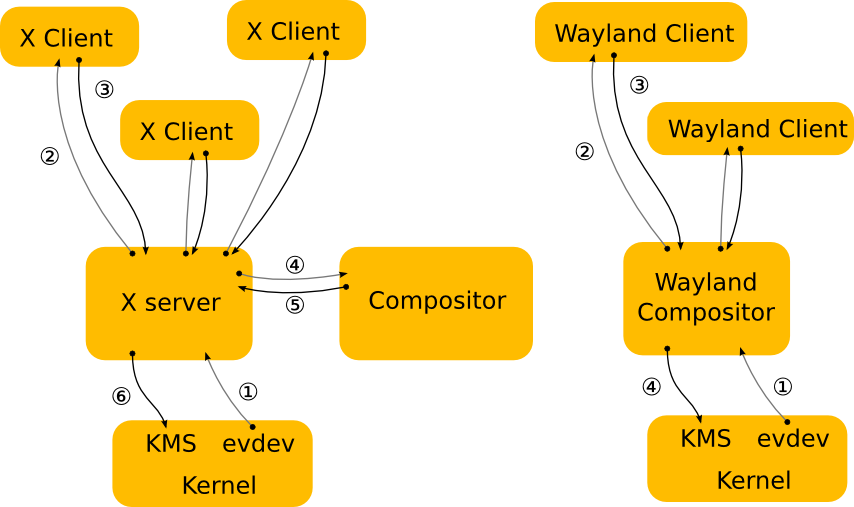
\includegraphics[width=1.0\textwidth]{images/wayland-x-architecture.png}
\caption{High level architecture of the X and Wayland windowing systems. Note that the X compositor is a separate entity from the display server, whereas the Wayland compositor provides the functionality of the display server internally. Image taken from  \protect\cite{litime}}
\label{wayland-vs-x}
\end{figure}



As illustrated in Figure \ref{wayland-vs-x}, the high level operation of the two windowing systems is largely the same, and the interface between the kernel and the display server are recycled, allowing Wayland to reuse much of the infrastructure developed to support X. The key difference that is relevant to this thesis, immediately visible in in Figure \ref{wayland-vs-x}, is Wayland’s integration of the display server and the compositor. 

In the X architecture, the compositor is a client, just like the applications, that communicates with the display server over the display server protocol. When clients send their output to the display server it is forwarded to the compositor, which composites the output based on its internal scenegraph of how the windows are laid out (which can, in the case of some compositors like Compiz, contain 3D window transformations), and sends this composited output back to the display server, which then draws it to the display. The key problem here is that the X server has its own internal representation of how the windows are laid out (which is strictly two dimensional), and when it receives input events from the kernel it  determines which window to deliver them to based on the location of the event and its own internal layout of the windows, rather than letting the compositor control the input event redirection. This means that if the compositor applies a 3D transformation to the window, this is not reflected in the X server’s internal window layout and so input events are not redirected to the appropriate client or transformed correctly into the client’s window space, making it essentially impossible to interact with windowed X applications in a meaningful way when they are embedded in a 3D space. 

In the Wayland architecture, by contrast, the compositor and the display server are the same entity and therefore by definition share an internal representation of how the windows are laid out. This allows the compositor to give windows an arbitrary embedding in a 3D space and still deliver input events to the applications driving them in a meaningful way. It also means that input events do not necessarily need to be delivered based on the embedding of the window surface itself, but can be delivered based on the embedding of an arbitrary spatial data structure associated with the surface, which is critical to the way the windowing system presented in this thesis handles 3D applications, since the output is drawn on a 2D surface but the interaction space the user perceives the user perceives for the application is three dimensional.

\section{Human Perception of Three Dimensions}

An important part of this thesis, and computer graphics in general, is exploiting the way that humans perceive three dimensional space to give them the illusion of 3D structure with 2D images. This may appear simple at a high level, since the human eye can only sense two dimensional images, but the way that humans use these 2D images to reconstruct the 3D structure of reality is extremely sophisticated and this makes the process of generating a compelling illusion much more complicated. Humans rely on a number of behaviors in the way the 3D structure of reality is projected to two dimensions by their eyes, called ‘depth cues’, to inform their understanding of the 3D structure of the scene they are observing.
	
There are many of these depth cues and, to the authors knowledge, no graphical system is capable of presenting all of them consistently to the user, but it is important for proper 3D perception that those cues which are present are consistent with one another and consistent between different parts of the scene. Because the windowing system presented in this thesis attempts to combine the output from different 3D applications into a cohesive 3D scene while still allowing these applications to control the projection of their 3D content to 2D, the synchronization of the parameters which control these depth cues between the compositor and the client applications is an important part of the work presented here. A brief overview of some of the relevant depth cues in included here to ensure all readers are familiar with the mechanism that enables them, as this is needed to understand the way the windowing system presented here creates the illusion of a consistent 3D scene composed of multiple 3D clients. The focus of this section is on depth cues which are handled by the windowing system presented here, for a more comprehensive and in depth discussion of depth cues in general, readers are directed to [citation].

\subsection{Motion Parallax and Stereopsis}

A key property of three dimensional space that allows us to perceive its structure from two dimensional images is that imaging the same 3D scene from different points in space results in different 2D images. Should this not be immediately apparent to the reader they are invited to hold their hand at arms length, move their head around, and observe how the portion of the scene which is occluded by their hand changes in response to the movement of their head. This effect, called ‘parallax’ forms the base of two very important and closely related depth cues: motion parallax (the change in projection based on the position and orientation of the users head), and stereo parallax or ‘stereopsis’ (the difference in the projection between the user’s eyes due to their slightly different location in space). On the hardware side, achieving the former requires that the system actively measure the position of the user’s head (called ‘head tracking’), and achieving the latter requires that the system be able to display a different image to each of the user’s eyes (making it a so called ‘stereo display’), and these two capabilities together form the requirements set forth in Section {Immersive 3D Displays} for and ‘immersive 3D display’. On the software side, the position of the virtual camera is controlled by the content of the view matrix (as explained in Section {The Vertex Transform}) , and so stereopsis requires that there be a separate view matrix for each eye (and that the scene is projected separately for each of these matrices) and motion parallax requires that these matrices change in response to changes in the user’s measured head transform.

Maintaining consistency is the effects of stereopsis and motion parallax between the compositor and all of its 3D client applications requires that all entities involved projecting 3D geometry do so with the same view matrices for each eye, and so an important part of the Wayland protocol extensions presented here is providing 3D clients with up to date view matrices for each eye before each frame is drawn, and giving the clients a mechanism for providing the compositor with different output for each of the user’s eyes.

\subsection{Relative Size}

Relative size refers to the change in the size of the projection of an object as it’s distance from the viewer changes, with objects appearing smaller to the viewer as they recede further into the distance. This behavior is achieved with, and is the primary purpose of, the projection matrix discussed in Section {The Vertex Transform}, which maps the frustum of space visible from the camera position (called the view frustum) onto the cubic region of space defined by the normalized device coordinates. Because the portion of the view frustum that is closer to the camera position is narrower than the portion which is further away, the process of mapping it into normalized device coordinates compresses geometry in the view frustum more the further it is from the camera position, making this geometry smaller the further it is from the camera, creating the illusion of relative size. In order to maintain the consistency in the relative size cue between all of the client applications and the compositor, it is necessary that all parts of the windowing system doing 3D projection do so using the same projection matrix, which is an important part of the display server protocol extensions presented here.

\subsection{Occlusion}

Another important, and familiar, aspect of three dimensional space is that when imaged onto a two dimensional plane, portions of the scene which are closer to the camera can hide, or ‘occlude’, portions that are further away. This gives us a powerful depth cue, because the occlusion of an object by another immediately tells us that the second object is closer, and the portion of the object that is occluded gives us even more detailed information about their spatial relation. As explained in Section {Rasterization and The Depth Test}, this behavior is achieved in the graphics pipeline by maintaining a 2D buffer containing the depth of each pixel, and only drawing a new pixel if it closer than the contents of the depth buffer. While this technique is both efficient and effective, using it to composite 3D content from multiple clients requires that the compositor have access to not only its own depth buffer, but also the depth buffers of all the 3D clients, and so providing a mechanism that allows this is an important part of the Wayland extensions presented here. 


\chapter{Design: A Unified Windowing System}
The core goal of this thesis is to demonstrate, both conceptually and practically, that windowing systems are capable of solving the same problems for 3D user interfaces that they currently solve for 2D user interfaces, that a single windowing system can solve the same problems for 2D and 3D interfaces, and that a system which does so can be built on top of an existing windowing system. To understand this further, let’s examine abstractly the services that a windowing system provides and how these map onto 3D interfaces.

\section{Windowing System Services}

In general, windowing systems provide a software platform for graphical applications that gives these applications a means to use the hardware resources they need to provide graphical interfaces without needing to interact with the hardware directly. Because the windowing system handles the direct interactions with the hardware, it is able to multiplex the use of hardware resources between many individual applications which need the capabilities they provide. Because providing these hardware capabilities to applications abstractly is the core purpose of the windowing system, it is important to understand what it is that they represent.

\subsection{Graphical Interface Hardware and The Graphical Interface Space}

Consider the interface hardware needed to provide a traditional, two dimensional, WIMP interface (and thereby needed to support a traditional windowing system). There are three essential components: a display, a mouse, and a keyboard. The display provides a two dimensional space in which two dimensional images can be drawn, and  the mouse allows limited symbolic input at any point in this two dimensional space. Together these two devices create a two dimensional spatial interface, two dimensional input and output in the same two dimensional space. 

The extension of this concept to three dimensions requires the ability of the hardware system to support three dimensional input and three dimensional output in the same three dimensional space, creating a proper three dimensional spatial interface. Immersive 3D displays provide the user with a compelling illusion of a three dimensional space which the computer can fill with arbitrary 3D content, and 3D input devices can be used to provide 3D input in this space, so existing, consumer grade 3D interface hardware can provide such a 3D interface space in the same way that a mouse and traditional display provide a 2D interface space. If the choice of 3D input device is restricted to hand held tracking devices with buttons, like the Razer Hydra used in the implementation presented here, then the 3D input set it provide is very closely analogous to the 2D input set provided by a traditional mouse: symbolic input from a few buttons coupled with continuous spatial tracking throughout the interface space.

The keyboard allows the user to give the computer complex symbolic input, but there is no spatial information attached to this input, and it is up to the software system to determine which region of the interface space, if any, that this input is delivered to. The keyboard itself is not related to the number of dimensions (or any other aspect) of the interface space, and this means that it can continue to serve its purpose in a 3D interface without needing to undergo any changes to its hardware design.

\subsection{Interface Contexts Within the Graphical Interface Space}
	


\section{Three Dimensional Windows With Two Dimensional Buffers}
\subsection{View And Projection Matrices}
\subsection{Stereo Color Buffers}
\subsection{Depth Buffers}
\subsection{Clipping}
\chapter{Implementation}
\label{sec:implementation}
This section describes the implementation of the design discussed in Section~\ref{sec:design} built on top of the Wayland display server protocol. This implementation, called `Motorcar`, is free and open source and available on GitHub \cite{motorcar-github}. It is intended both to demonstrate concretely that such a design is practical to implement, as well as to serve as a functional 3D windowing system and provide a modular core of that can form the basis of further research into the concept of 3D windowing systems.

\section{Wayland Protocol Extensions}

The design outlined in Section~\ref{sec:design} requires several pieces of functionality not provided by the core Wayland protocol (like synchronization of the view and projection matrices between the compositor and the clients) and functionality that is not supported by the subsystems on which Wayland in built (like the ability for the compositor to access client depth buffers)



% ------------- End main chapters ----------------------

\clearpage
\bibliographystyle{plain}
\bibliography{Bibliography}
%\addcontentsline{toc}{chapter}{Bibliography}

%\begin{appendix}
%%\addcontentsline{toc}{chapter}{\appendixnamelower}
%\include{Appendix}
%\end{appendix}

\end{document}